\section{Random Number Generator Package}
To expand the techniques available in BNumMet even further, we will incorporate a lesser-known field of numerical methods, namely the implementation of generators for (pseudo) random numbers. The underlying motivation for its development is our interest about how random number generators function, as well as allowing the end-user to study a side of numerical techniques that is not generally taught. We should also mention that this package was not originally intended to be developed, but due to some extra time, we decided it would be beneficial to include it.

Many of the suggested techniques rely on specific values being initialized, so we used a Python dictionary to help students understand the meaning of each variable by associating a key with its value; this dictionary is then used as a global dictionary in the appropriate method.

In this section the following algorithms had been implemented by the author of this work:
\begin{itemize}
    \item Lehmers Random Number Generator \algoref{alg:lehmersrand}
    \item Marsaglia Random Number Generator \algoref{alg:Marsaglia Random Number Generator Algorithm}
    \item Mersenne Twister Random Number Generator \algoref{alg:Mersenne Twister Random Number Generator}
\end{itemize}

\subsection{Lehmer's Generator}
Lehmer's Random Number Generator is one of the simplest yet most elegant generators available. This type of generator is a Linear Congruential generator, which is defined by the following recurrence relation~\cite{payne1969coding,park1988random}.
\[x_{n+1} = k\cdot x_n \mod{n}\]

In the case of Lehmer's generator it follows:
\[x_{n+1} = (a\cdot x_n+c) \mod{n}\]
The selection of $a,c,n$ and $x_0$ is critical, and some values have been proposed for optimal generation; one of these values has been used as the method's default initializer, in particular:
\[a= 7^5, c=0, m=2^{31}-1, x_0 = 1 \]

These values ensure that this generator works properly, but some bad generators can be found, which is an interesting exercise for the student to search for or come up with. Additionally it is worth mentioning that the developped function allows for input parameters to be set.

The algorithm implementation was based upon Moller's work~\cite{doi:10.1137/1.9780898717952}.
\subsubsection{Examples}
	\paragraph{Example 1}{
\begin{lstlisting}[language=Python]
from BNumMet.Random import lehmers_rand
for i in range(10):
    print(lehmers_rand())

>> Lehmers Random Number Generator Initialized with default values
	a=16807
	c=0
	m=2147483647
	x=1.0
    7.826369259425611e-06
    0.13153778814316625
    0.7556053221950332
    0.4586501319234493
    0.5327672374121692
    0.21895918632809036
    0.04704461621448613
    0.678864716868319
    0.6792964058366122
    0.9346928959408276
\end{lstlisting}
}
\paragraph{Example 2: Predictability of Lehmer's Random Number Generator}{
\begin{lstlisting}[language=Python]
from BNumMet.Random import lehmers_rand, clear_lehmers_vars
clear_lehmers_vars()
arr = [1]
for i in range(10):
    aux = lehmers_rand(a=2**16 + 3, m=2**31, c=0, x=arr[-1])
    if len(arr) >= 3:
        lehmerFormula = (6 * arr[-1] - 9 * arr[-2]) % 1  # Test Xn = (6Xn-1 - 9Xn-2)
        print(f"Lehmer's = {aux}\nPredicted = {lehmerFormula}\n")
    arr.append(aux)

>>  Lehmer's = 0.0008239871822297573
    Predicted = 0.0008239871822297573
    
    Lehmer's = 0.003295936156064272
    Predicted = 0.003295936156064272
    
    Lehmer's = 0.012359732296317816
    Predicted = 0.012359732296317816
    
    Lehmer's = 0.04449496837332845
    Predicted = 0.04449496837332845
    
    Lehmer's = 0.15573221957311034
    Predicted = 0.15573221957311034
    
    Lehmer's = 0.533938602078706
    Predicted = 0.533938602078706
    
    Lehmer's = 0.8020416363142431
    Predicted = 0.8020416363142431
    
    Lehmer's = 0.006802399177104235
    Predicted = 0.006802399177104235
\end{lstlisting}
}
\paragraph{Example 3: Visual failure}{
\begin{lstlisting}[language=Python]
from BNumMet.Random import lehmers_rand, clear_lehmers_vars
clear_lehmers_vars()
fail2 = (
    lambda: float(
        (int(lehmers_rand(a=65539, c=0, m=2**31, x=123) * (2**31)) >> 23) & 0xFF
    )
    / 255
)
fail = [(fail2(), fail2()) for i in range(100000)]
plt.scatter(*zip(*fail), s=1, c="black")
plt.show()
\end{lstlisting}
\begin{figure}[H]
    \centering
    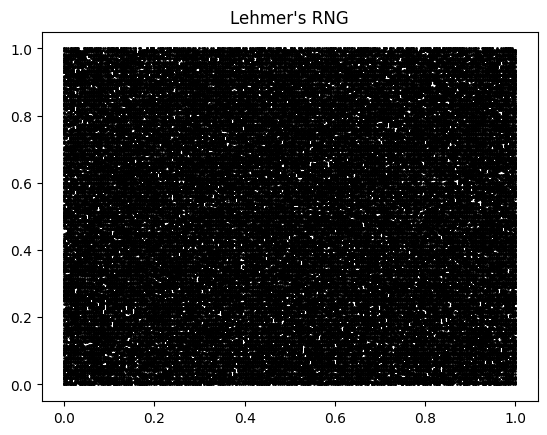
\includegraphics{Include/Images/Thesis/Documentation/Randomness/Lehmers Rand Example 3.png}
    \caption{Lehmers Rand Example 3}
    \label{fig:Lehmers Rand Example 3}
\end{figure}
}



\subsection{Marsaglia's Generator}

In the original paper~\cite{10.1214/aoap/1177005878} Marsaglia expands on random number generators by providing a generator that is born from a type of relation such as Fibonacci, those generators that add or subtract previous values from the current value, but in Marsaglia's case this generator has some \textit{lag} added to it, that is it extends the appearance of the value that would be expected without \textit{lag}. It is accomplished by introducing two parameters know as $lag_s$ and $lag_r$ as well as a $carry$ variable which will be $1$ if the generated number is negative - to which the $base$ will be added - and $0$ if the generator produced a positive number. This $carry$ variable is what gives the name to this type of generator which are known as $add-with-carry$ or $subtract-with-borrow$

One of the complexities of this method is that it generates primarily integer numbers and is limited to the base it accepts as input; however, dividing by the base (the largest number in the generator) produces a decimal number between 0 and 1. Some input arguments were proposed, but as we saw in Lehmer's generator, some default parameters were provided. 
\[base = 2^{31}-1, lag_r=19, lag_s=7, carry=1, seed\_tuple = (1,1)\]
This set of values was proposed in the original paper; it is also worth noting that we used the subtract with borrow method, despite the fact that the addition with carry method is analogous. We strongly encourage students to try to find ill-inputs that generate patterns in their output.

We have implemented the algorithm using the original approach of Marsaglia~\cite{10.1214/aoap/1177005878}.
\subsubsection{Examples}
	\paragraph{Example 1}{
\begin{lstlisting}[language=Python]
from BNumMet.Random import marsaglia_rand, clear_marsaglia_vars
clear_marsaglia_vars()
for i in range(10):
    print(marsaglia_rand(base=41, lag_r=2, lag_s=1, carry=0, seed_tuple=(0, 1)))

>>  0.975609756097561
    0.024390243902439025
    0.926829268292683
    0.0975609756097561
    0.8048780487804879
    0.2926829268292683
    0.4878048780487805
    0.8048780487804879
    0.6585365853658537
    0.12195121951219512
\end{lstlisting}
}
\paragraph{Example 2}{
\begin{lstlisting}[language=Python]
from BNumMet.Random import marsaglia_rand, clear_marsaglia_vars
clear_marsaglia_vars()
fail = [
    (
        marsaglia_rand(base=100, lag_r=2, lag_s=1, carry=0, seed_tuple=(0, 1)),
        marsaglia_rand(base=100, lag_r=2, lag_s=1, carry=0, seed_tuple=(0, 1)),
    )
    for i in range(100000)
]
plt.scatter(*zip(*fail), s=1, c="black")
\end{lstlisting}
\begin{figure}[H]
    \centering
    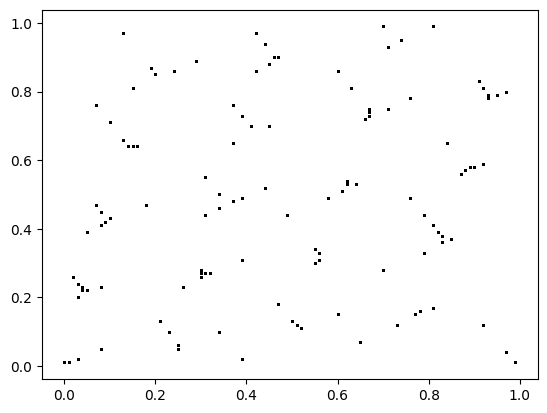
\includegraphics{Include/Images/Thesis/Documentation/Randomness/Marsaglia Rand Example 2.png}
    \caption{Marsaglia Rand Example 2}
    \label{fig:Marsaglia Rand Example 2}
\end{figure}
}
\paragraph{Example 3}{
\begin{lstlisting}[language=Python]
from BNumMet.Random import marsaglia_rand, clear_marsaglia_vars
clear_marsaglia_vars()
fail = [
    (
        marsaglia_rand(base=41, lag_r=2, lag_s=1, carry=0, seed_tuple=(0, 1)),
        marsaglia_rand(base=41, lag_r=2, lag_s=1, carry=0, seed_tuple=(0, 1)),
    )
    for i in range(100000)
]
plt.scatter(*zip(*fail), s=1, c="black")
\end{lstlisting}
\begin{figure}[H]
    \centering
    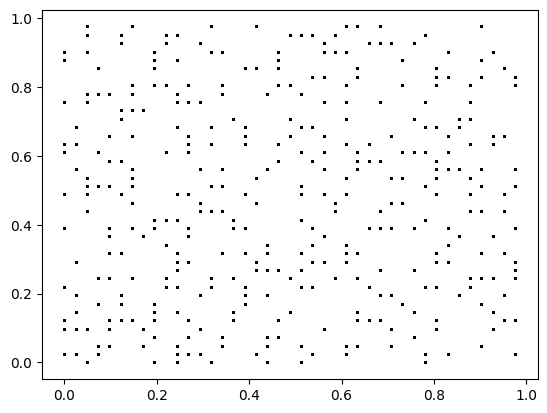
\includegraphics{Include/Images/Thesis/Documentation/Randomness/Marsaglia Rand Example 3.png}
    \caption{Marsaglia Rand Example 3}
    \label{fig:Marsaglia Rand Example 3}
\end{figure}
}



\subsection{Mersenne Twister Generator}
The Mersenne Twister is an algorithm first introduced by Makoto Matsumoto and Takuji Nishimura~\cite{matsumoto1998mersenne}. According to the creators, the choice of parameters may produce a period (repetitions of random numbers) of $2^{19937}-1$ while only requiring 624 words of memory and every word is made up of 32 bits - on the original implementation, newer ones exists with 64 bits. Most notably, it is the most often used generator, serving as the default generator for the Python and R programming languages.

We opted to implement the technique due to its popularity, even if the mathematics behind it are outside the scope of this project. We reckon the code is simple and does not require a lot of focus to comprehend what it is doing. Furthermore, we wanted to give students with commonly utilized approaches, and the Mersenne Twister is unquestionably one of them.

As Makoto and Takuji did, they ran a battery of tests to prove the generation of random numbers; similarly, we will assess the efficacy of this method.

The implementation of the method was based upon the original work~\cite{matsumoto1998mersenne} which contains a C implementation.
\subsubsection{Analysis of solution}
One question that arises in Random Number Generators is, how can we make sure our generator is actually random?, in this section we will dive into how we have tested our Mersenne Twister function.

The reference we have followed is~\cite{smid2010statistical}, which develops a suite of tests to check different random number generators, and we have used an already developed version of this suite for Python~\cite{InsaneMonster2022}, since it was out of the scope of this project. 

Some discussion of the test we are eligible to test are the following.


\begin{enumerate}
\item  \textbf{Monobit test}: This test purpose is to count how many zeros are there in the sequence, if it is close (up to some epsilon) to ½ then the tests will pass. This is a crucial test inside the suite since if this test fails, the rest will not pass.

\item  \textbf{Frequency within a Block: }The test is analogous to the Monobit but instead of counting number of zeros in the entire string, it counts the frequency of 1 appearing in M-sized blocks, it should be close to M/2 plus or minus epsilon. 

\item  \textbf{Runs Tests: }This test counts the number of runs the sequence has. A run of length \textit{k} consists of exactly \textit{k} identical bits and is bounded by a bit of opposite value. 

\begin{enumerate}
\item  ``01111110'' : Run of length 6
\end{enumerate}


If the lengths are the ones one could expect from a random number, then the test will pass.


\item  \textbf{Longer Runs Test}: In this case, the goal is to determine if the longest run length of ones is consistent with what one can expect from a random number.  An irregularity in the length of ones, implies an irregularity in the length of zeros.

\item  \textbf{Discrete Fourier Spectral Test}: It tries to detect periodic features of the run, it applies the Discrete Fourier Transform and count the peaks, the main goal is to find if the peaks that exceed the 95\% threshold are less than 5\%.

\item  \textbf{Non-overlapping Template Matching:} The test tries to find generators that produce many occurrences of a aperiodic pattern, it searches on blocks of m bits for these types of patterns.

\item \textbf{ Serial test}: This test focuses on determining the number of occurrences of the $2^m$ length of bit patterns and checking if they are one that is to be expected, since random sequences have uniformity, so each sequence has the same probability of appearing. Were we to take $m=1$ we would have the same results as in the monobit test.

\item  \textbf{Approximate Entropy Test: }This is exactly the serial test, but compares with 2 consecutive blocks of lengths $m$ and $m+1$.

\item \textbf{ Cumulative sums: }This test tries to find which is the maximal length of a random walk, assuming a $0\ =\ -1$ and summing all the sequence, it should be close to zero.

\item \textbf{ Random Excursion: }It checks that the number of cycles that have k visits in a cumulative sum walk is that of a properly random test.

\begin{enumerate}
\item A cycle consists of a sequence of steps taken at random that begin at and return to the origin.
\end{enumerate}

\item \textbf{ Random Excursions Variant Test: }Counts how many times a particular state is visited in a random cumulative sum.
\end{enumerate}

\paragraph{Results}
To test it we will generate a total of 100 random integer numbers and run the battery of test through that sequence.
\begin{lstlisting}[language=Python]
import numpy
from nistrng import *

clear_mt_vars()
# Test genrand from nistrng
sequence = numpy.array([genrand() * 0xFFFFFFFF for i in range(100)], dtype=numpy.uint64)


binary_sequence: numpy.ndarray = pack_sequence(sequence)

# Check the eligibility of the test and generate an eligible battery from the default NIST-sp800-22r1a battery
eligible_battery: dict = check_eligibility_all_battery(
    binary_sequence, SP800_22R1A_BATTERY
)
for i in eligible_battery:
    #print(i)
    ...

# Test the sequence on the eligible tests
results = run_all_battery(binary_sequence, eligible_battery, False)
# Print results one by one
for test,(res,_) in zip(eligible_battery,results):
    print(f"Test: {test} \n\tResult: {res.passed}")

>> Initialized the global dictionary mtVars with seed 4357
    Test: monobit 
    	Result: True
    Test: frequency_within_block 
    	Result: True
    Test: runs 
    	Result: True
    Test: longest_run_ones_in_a_block 
    	Result: True
    Test: dft 
    	Result: True
    Test: non_overlapping_template_matching 
    	Result: True
    Test: serial 
    	Result: True
    Test: approximate_entropy 
    	Result: True
    Test: cumulative sums 
    	Result: True
    Test: random_excursion 
    	Result: False
    Test: random_excursion_variant 
    	Result: True
\end{lstlisting}

The results are positive, except for one, on closer investigation it seems like this test suite has one flaw [\href{https://github.com/InsaneMonster/NistRng/issues/9}{https://github.com/InsaneMonster/NistRng/issues/9}] documented by one of the users, after the change they suggested it works and outputs True. Therefore, a success in all test, we can assure our students that the Mersenne Twister is a true random number generator.

\subsubsection{Examples}
	\paragraph{Example 1}{
\begin{lstlisting}[language=Python]
from BNumMet.Random import clear_mt_vars,genrand
clear_mt_vars()
for i in range(10):
    print(genrand())

>>  Initialized the global dictionary mtVars with seed 4357
    0.8173300600185361
    0.9990608997175147
    0.5103543725587322
    0.13153290984489324
    0.03541634837990076
    0.9924695345089932
    0.6257087035630151
    0.06259194576707482
    0.4107105111262553
    0.13477367491805314
\end{lstlisting}
}
\paragraph{Example 2}{
\begin{lstlisting}[language=Python]
from BNumMet.Random import clear_mt_vars,genrand
clear_mt_vars()
toPlot = [(genrand(),genrand()) for i in range(100000)]
plt.scatter(*zip(*toPlot), s=1, c="black")
\end{lstlisting}
\begin{figure}[H]
    \centering
    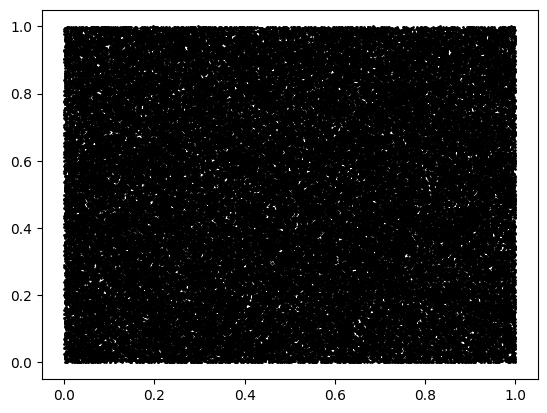
\includegraphics{Include/Images/Thesis/Documentation/Randomness/MersenneTwister Rand Example 2.png}
    \caption{Mersenne Twister Rand Example 2}
    \label{fig:Mersenne Twister Rand Example 2}
\end{figure}
}
